\section{Experiments}

\begin{savenotes}
\begin{table*}[h]
\begin{center}
%\scriptsize
\caption{Tests on Selected Benchmarks}\label{table:benchmarks}
     \begin{threeparttable}
     %\def\arraystretch{1.2}
\begin{tabular}{c|c|c|c|c|c|c|c|c|c|c|}
		\cline{2-11}	  
& \multicolumn{3}{c|}{Test Programs} & \multicolumn{5}{c|}{Symbolic Model Checking} & \multicolumn{2}{c|}{Other Tools} \\ \cline{2-11}   
        & $Name$ & \#P & \#Calls & $k$ & \#Match & $\mathrm{SMT_{OAMP}}$ Tm & $\mathrm{SMT_{UAMP}}$ Tm & Speed & ISP Tm & MOPPER Tm \\ \hline
         \multicolumn{1}{ |c|  }{\multirow{5}{*}{\rotatebox[origin=c]{90}{AssertV}}} 
          &  \textit{Diffu2DNoBa}\tnote{d} & 16 & 188 & 3 & 1,066  & 51.543s & 87.361s& 0.59 & TO & N/A\\ \cline{2-11}
         \multicolumn{1}{ |c|  }{}&  \textit{DeepComm} & 5 & 180 & 1 & 240 & 1378.539s & 0.837s& 1,647 & TO & N/A \\ \cline{2-11}
\multicolumn{1}{ |c|  }{}&  \textit{Pktuse} &5 & 2048 &1 & 1,792 & TO & 180s & $>$40\tnote{b}  & TO & N/A \\ \cline{2-11}
\multicolumn{1}{ |c|  }{}&  \textit{MultiM} & 3 & 266 & 1 & 500  & 3213.140s & 10.892s & 295 & TO & N/A\\ \cline{2-11}
\multicolumn{1}{ |c|  }{}&  \textit{Floyd}\tnote{d} &32 & 528 & 2 & 1,928  & 29.062s & 60.546s & 0.48 & TO & N/A\\ \hline
\hline
        
	         \multicolumn{1}{ |c|  }{\multirow{7}{*}{\rotatebox[origin=c]{90}{ZeroCom}}} 
         &  \textit{MonteCarlo} & 16 & 155 & 1 & 241  & 2.494s & 1.875s & 1.33 & TO & 3.019s \\ \cline{2-11}
% \multicolumn{1}{ |c|  }{} &  \textit{Diffu2DNoBa}\tnote{d}& 16 & 188 & 3& 1,066 & 5.394s & 10.177s & 0.53 & & \\ \cline{2-11}
        \multicolumn{1}{ |c|  }{} &  \textit{DeepComm} & 5 & 180 & 1 & 240 & 254.625s & 0.875s& 291 & TO & TO \\ \cline{2-11}
\multicolumn{1}{ |c|  }{}&  \textit{Pktuse} &5 & 2048 &1 & 1,792 & TO & 121s & $>$59\tnote{b} & TO & 565.857s \tnote{a} \\ \cline{2-11}
\multicolumn{1}{ |c|  }{}&  \textit{MultiM} & 3 & 266 & 1 & 500  & 3042.192s & 8.312s & 366 & 20.334s & 16.590s \\ \cline{2-11}
\multicolumn{1}{ |c|  }{}&  \textit{Mismatch} &3 & 800 &1 & 204 & 8.886s & 2.904s & 3.06 & 483.128s & 14.539s \\ \cline{2-11}
\multicolumn{1}{ |c|  }{}&  \textit{MismatchEx} &3 & 296 &1 & 165 & 507.204s & 0.579s & 876 & TO & N/A \tnote{+} \\ \cline{2-11}
\multicolumn{1}{ |c|  }{}&  \textit{Floyd} &32 & 528 &1 & 1,928 & 90.812s & 89.032s & 1.02 & TO & 166.477s\\ \hline
\hline

         \multicolumn{1}{ |c|  }{\multirow{6}{*}{\rotatebox[origin=c]{90}{DL}}} 
         &  \textit{Diffu2DNoBa} & 16 & 188 & 1 & 514  & 46.967s & 3.479s & 13.50 & TO & TO\\ \cline{2-11}
          \multicolumn{1}{ |c|  }{}  &  \textit{Heat} & 16 & 312 & 1 & 184 & 2.728s & 0.963s  & 2.83 & TO & 2.976s \\ \cline{2-11}
 \multicolumn{1}{ |c|  }{}  &  \textit{Integrate}\tnote{d} & 16 & 76 & 1 & 240  & 0.056s & 0.052s & 0.93 & TO & TO \\ \cline{2-11}
  \multicolumn{1}{ |c|  }{}  &  \textit{IS}\tnote{d} & 256 & 508 & 1 & 255 & 0.127s & 0.109s & 1.17 & 453.764s & 11.326s \\ \cline{2-11}
\multicolumn{1}{ |c|  }{}&  \textit{Mismatch} &3 & 800 &1 & 204  & 14.278s & 2.160s & 6.61 & 514.852s & 17.892s\\ \cline{2-11}
\multicolumn{1}{ |c|  }{}&  \textit{MismatchEx} &3 & 296 &3 & 328  & 34.119s & 1.253s & 27.23 & TO & N/A \tnote{+} \\ \hline 
\end{tabular}
\begin{tablenotes}
\item[d] The property does not exist for the benchmark.
\item[a] The test terminates unexpectedly with out of memory.
\item[b] The number is not concrete as the test with the over-approximated match pairs is time out. 
\item[+] MOPPER is not launched because the process of trace generation finds a deadlock.
%\item[+] The precise match pairs are over-approximated as $k$ is reached.
\end{tablenotes}
     \end{threeparttable}
\end{center}
\end{table*}
\end{savenotes}

This section describes a series of experiments over a set of benchmarks to determine (1) how quickly the properties of the input program are uncovered, and (2) how well the algorithm controls the size of the match pair set as the bound $k$ increases.

The benchmark programs are specific to the Message Passing Interface (MPI), a widely used message passing standard \cite{mpi3.1}, and come from different sources. Seven are derived from actual MPI programs and are used in other works for benchmarking \cite{benchmark:fevs,mpptest_benchmark,DBLP:conf/ppopp/XueLWGCZZV09,benchmark:mentoCarlo,Mueller:SC2011,Bailey1991}.

\begin{compactitem}

\item \textit{Diffu2DNoBa} is modified from the program \textit{Diffusion 2D}, which uses barriers to “partition” the message communication into several sections \cite{benchmark:fevs}. \textit{Diffu2DNoBa} removes the barriers from the original program so deadlocks are present in the new program. The program is also interesting because the messages to any receiver are distributed from a large set of senders.

\item \textit{Pktuse} is executed with 5 processes -- each of which has a long sequence of messages to be sent to the other processes \cite{mpptest_benchmark}. The program uses wildcard receives only, therefore has a high degree of message non-determinism. 

\item \textit{Floyd} implements the shortest path algorithm for all the pairs of nodes \cite{DBLP:conf/ppopp/XueLWGCZZV09}. Each node communicates only with the immediate following neighbor. The program also has a large set of senders for each receiver. 


\item \textit{MonteCarlo} \cite{benchmark:mentoCarlo} implements the Monte Carlo method by a master-slave model. The program has a deadlock trace under the zero buffer setting.

\item \textit{Integrate} \cite{benchmark:fevs} implements the algorithm that computes an integral of the $\sin$ function by using a large number of wildcard receives to match the sends from multiple sources.

\item \textit{Heat} \cite{Mueller:SC2011} implements the solution of the heat conduction equation. The communication pattern for this benchmark contains several orphaned receive deadlocks.

\item \textit{IS} \cite{Bailey1991} implements the solution of integer sorting. The message passing in this benchmark is deterministic.
\end{compactitem}

The remaining four are synthetic programs created for this study.

\begin{compactitem}
\item \textit{DeepComm} is a simple program with one receiver and 4 senders. The program is designed to have a long sequence of sends in each sender.
Also, this scenario issues only wildcard receives, so that the messages from different senders may race.

\item \textit{MultiM} is an extension to a program in the MCAPI library distribution.
%\cite{DBLP:conf/kbse/HuangMM13}. 
The program adds extra iterations to the original program to generate longer execution traces. The program uses only wildcard receives and is designed to have an interesting violation of assertion that only occurs in some possible executions.

\item \textit{Mismatch} is designed to contain a communication deadlock in execution. The program interleaves wildcard receives and deterministic receives in the program text. A deterministic receive may be orphaned in program execution leading to a deadlock as all the potential sends it needs are matched with the preceding wildcard receives. 

\item \textit{MismatchEx} is an extension to the program in \figref{fig:example} that contains more sends and receives. Similar to the program in \figref{fig:example}, a deadlock may occur in deep execution. 
%No assertions are present in the program.
\end{compactitem}


These programs are tested for three types of properties: assertion violation, zero buffer compatibility and deadlock. 
Each program is tested under four environments of analysis showing the comparison of time cost. 
``$\mathrm{Symbolic\ Model\ Checking}$'' shows the SMT solution with two algorithms of match pair generation .
``$\mathrm{Other\ Tools}$'' are the state-of-the-art MPI verifiers including the dynamic analyzer ISP \cite{DBLP:conf/ppopp/VakkalankaSGK08} and the deadlock analyzer MOPPER\cite{DBLP:conf/fm/ForejtKNS14,DBLP:journals/toplas/ForejtJKNS17}. 
ISP is a general verification tool for message passing programs.
MOPPER is a trace based verifier that is specific to deadlock and zero buffer compatibility. Therefore, the assertion violation tests are not available for MOPPER.
%The deadlock checking relies on a static pattern matcher to identify potential deadlock scenarios \cite{deadlock-draft}. 
%The experiments here use single pattern match, and the SMT encoding is to witness the feasibility of that match. The same pattern match is used for all experiments on any given deadlock example. 
The initial program trace for symbolic model checking is generated by MPICH \cite{mpich}, a public implementation of the MPI standard.
The SMT encoding for each test 
%is generated by the existing rules \cite{DBLP:conf/kbse/HuangMM13,HuangNFM15} and 
is solved by Z3 \cite{demoura:tacas08}. 
The experiments are run on a AMD A8 Quad Core processor with 6 GB of memory running Ubuntu 14.04 LTS. 
A time limit of 2 hours is set for each test. The test aborts the verification process if it does not complete within the time limit.

\subsection{Effectiveness}


The \textit{effectiveness of property witnessing} are shown in \tableref{table:benchmarks} that divides the tests into three groups, where each group is the tests for a single type of property. Each group is labeled in the first column: ``AssertionV" means assertion violation; ``ZeroCom" means zero buffer compatibility; and ``DL" means deadlock. For each benchmark, ``\#P" is the number of processes in the tested program, ``\#Calls" is the total number of sends, receives, waits and collective operations.
$k$ is the ``optimal'' value at which the property is witnessed (if the property is satisfied), or the value at which the over-approximated match set is generated (if the property is not satisfied). 
The column ``\#Match" is the number of the generated match pairs for $k$. 
The column ``$\mathrm{SMT_{OAMP}\ Tm}$'' is the runtime of checking satisfiability with an over-approximation of match pairs \cite{DBLP:conf/kbse/HuangMM13}.
The column ``$\mathrm{SMT_{UAMP}\ Tm}$" is the cumulative sum: $\sum_{i=1}^k\mathrm{Tm}_i$, where $\mathrm{Tm}_i$ is the runtime of checking satisfiability with the under-approximated match pairs for the bound $i$.
%The notation ``TO" means ``time out" (exceeding the time limit set for each test). 
The column ``Speed" reports the relative speedup over ``$\mathrm{SMT_{OAMP}\ Tm}$'': $\mathrm{SMT_{OAMP}\ Tm} / \mathrm{SMT_{UAMP}\ Tm}$.
The column ``Tm'' for ISP is the running time of dynamic analysis. 
The column ``Tm'' for MOPPER is for constraint generation and solving.
The notation ``TO'' means ``time out'' (exceeding the time limit set for each test). 
The notation ``N/A'' means ``not available''.
%The symbol ``--" means that the $\mathrm{Speed}$ can not be computed because the test times out.

\begin{comment}

\begin{savenotes}
\begin{table*}[t]
\begin{center}
\scriptsize
\caption{Tests on Selected Benchmarks}\label{table:benchmarks}
     \begin{threeparttable}
     \def\arraystretch{1.5}
\begin{tabularx}{0.8\textwidth}{c|c|c|c|p{0.25cm}|c|c|c|p{0.25cm}|c|c|c|c|c|c|c|}
		\cline{2-16}	  
& \multicolumn{3}{c|}{Test Programs} & \multicolumn{4}{c|}{Test 1} & \multicolumn{4}{c|}{Test 2} & \multicolumn{4}{c|}{Test 3}  \\ \cline{2-16}   
        & $Name$ & \#P & \#OP & $k$\tnote{w} & \#M & Time & Speed& $k$ & \#M & Time & Speed & $k$\tnote{+} & \#M & Time & Speed\\ \hline
         \multicolumn{1}{ |c|  }{\multirow{5}{*}{\rotatebox[origin=c]{90}{AssertV}}} 
          &  \textit{Diff2DNoBa} & 16 & 188 & 1\tnote{d} & 514 & 3.508s & 14.86 & 2\tnote{d}& 934 & 31.722s & 1.48 & 3\tnote{d}& 1,066 & 52.131s & 0.59 \\ \cline{2-16}
         \multicolumn{1}{ |c|  }{}&  \textit{DeepComm} & 5 & 180 & 1 & 240 & 0.837s & 1,647 & 5 & 960 & 10.547s & 131 & 15 & 2,760 & 1,379s & 1.00 \\ \cline{2-16}
\multicolumn{1}{ |c|  }{}&  \textit{Pktuse} &5 & 2048 &1 & 1,792 & 180s & $>$40 & 5   &    4,828      & 564s & $>$13 & 128 & 99,328 & TO & -- \\ \cline{2-16}
\multicolumn{1}{ |c|  }{}&  \textit{MultiM} & 3 & 266 & 1 & 500 & 10.892s & 295 & 5 & 1,300 & 24.397s & 132 & 100 & 20,300 & 3,218s & 1.00\\ \cline{2-16}
\multicolumn{1}{ |c|  }{}&  \textit{Floyd} &32 & 528 &1\tnote{d}& 1,928 & 29.925s & 0.97 & 2\tnote{d} &    1,928      & 30.621s & 0.48 & 3\tnote{d} & 1,928 & 29.043s & 0.32 \\ \hline
\hline
        
         \multicolumn{1}{ |c|  }{\multirow{7}{*}{\rotatebox[origin=c]{90}{ZeroCom}}} 
         &  \textit{Diff2DNoBa} & 16 & 188 & 1\tnote{d} & 514 & 1.749s & 3.07 & 2\tnote{d} & 934 & 3.053s & 1.12 & 3\tnote{d}& 1,066 & 5.375s & 0.53 \\ \cline{2-16}
        \multicolumn{1}{ |c|  }{} &  \textit{DeepComm} & 5 & 180 & 1 & 240 & 0.875s & 291 & 5 & 960 & 3.056s & 83 & 15 & 2,760 & 255s & 1.00 \\ \cline{2-16}
\multicolumn{1}{ |c|  }{}&  \textit{Pktuse} &5 & 2048 &1 & 1,792 & 121s & $>$59 & 5   &    4,828      & 449s & $>$16 & 128 & 99,328 & TO & -- \\ \cline{2-16}
\multicolumn{1}{ |c|  }{}&  \textit{MultiM} & 3 & 266 & 1 & 500 & 8.312s & 366 & 5 & 1,300 & 17.843s & 170 & 100 & 20,300 & 3,043s & 1.00\\ \cline{2-16}
\multicolumn{1}{ |c|  }{}&  \textit{Mismatch} &3 & 800 &1 & 204 & 2.904s & 3.06 & 30   &    622      & 3.297s & 2.69 & 50 & 793 & 8.872s & 1.00 \\ \cline{2-16}
\multicolumn{1}{ |c|  }{}&  \textit{MismatchEx} &3 & 296 &1 & 165 & 0.579s & 876  & 20   &    1,687      & 7.433s & 68 & 43 & 3,525 & 507s & 1.00  \\ \cline{2-16}
\multicolumn{1}{ |c|  }{}&  \textit{Floyd} &32 & 528 &1 & 1,928 & 89.032s & 1.02 & 5   &    1,928      & 90.908s & 1.00 & 10 & 1,928 & 91.155s & 1.00 \\ \hline
\hline

         \multicolumn{1}{ |c|  }{\multirow{3}{*}{\rotatebox[origin=c]{90}{DL}}} 
         &  \textit{Diff2DNoBa} & 16 & 188 & 1 & 514 & 3.479s & 13.50 & 2 & 934 & 44.060s & 1.07 & 3 & 1,066 & 46.974s & 1.00 \\ \cline{2-16}
\multicolumn{1}{ |c|  }{}&  \textit{Mismatch} &3 & 800 &1 & 204 & 2.160s & 6.61 & 30   &    622      & 10.061s & 1.42 & 50 & 793 & 14.286s & 1.00 \\ \cline{2-16}
\multicolumn{1}{ |c|  }{}&  \textit{MismatchEx} &3 & 296 &3 & 328 & 1.253s & 27.23 & 20   &    1,687      & 2.438s & 13.99 & 43 & 3,525 & 34.116s & 1.00 \\ \hline

       
\end{tabularx}
\begin{tablenotes}
\item[w] $k$ is the minimum value with which the property is witnessed (if the property exists). 
\item[d] The property does not exist for the benchmark.
\item[+] The precise match pairs are over-approximated as $k$ is reached.
\end{tablenotes}
     \end{threeparttable}
\end{center}
\end{table*}
\end{savenotes}

\end{comment}

\examplefigtemplate

\begin{figure*}[h]
\centering
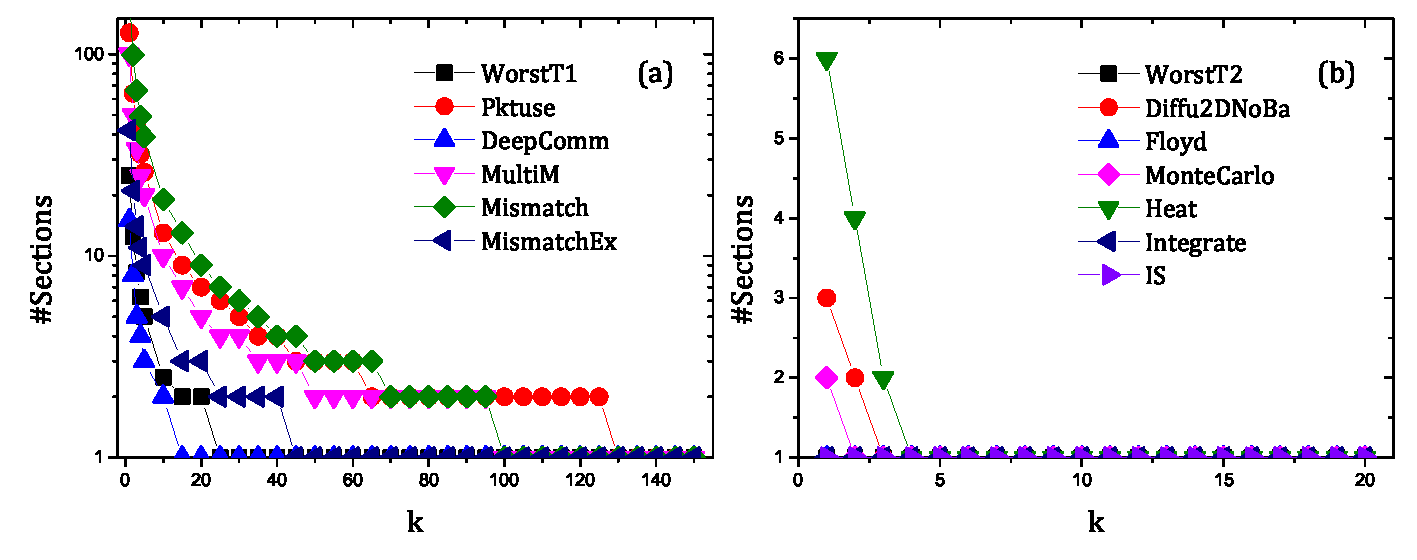
\includegraphics[scale=0.65]{fig/figure3a-3b_ex.eps}
\caption{The number of partitioned sections of varying the input $k$.}
\label{fig:relation:section}
\end{figure*}


\begin{figure*}[h]
\centering
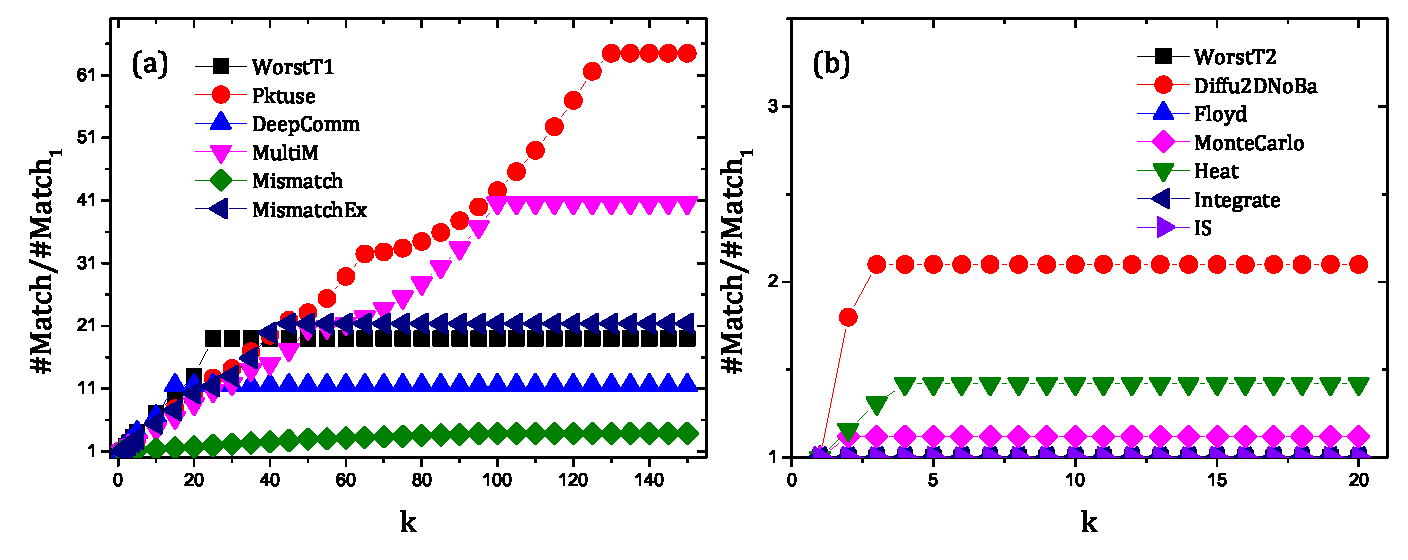
\includegraphics[scale=0.65]{fig/figure4a-4b_ex.eps}
\caption{The relative growth of the number of match pairs of varying the input $k$, where $\mathrm{Match}_1$ is the number of the generated match pairs for $k=1$.}
\label{fig:relation:match}
\end{figure*}

The results in \tableref{table:benchmarks} show that the symbolic model checking is obviously quicker than ISP and MOPPER in most tests. ISP is time out for most benchmarks because it has to explore massive schedules before witnessing a property. MOPPER is more efficient than ISP but still suffers from the scalability for some benchmarks such as \textit{DeepComm}, \textit{Diffu2DNoBa} and \textit{Integrate}. 
The symbolic model checking with over-approximated match pairs is able to scale to most benchmarks except for the benchmarks \textit{MultiM} and \textit{Pktuse}. 
The symbolic model checking with under-approximation of match pairs, in contrast, highly speeds up all the tests such that each test only takes less than one second on average.

The tested property, if existing in a benchmark, can be witnessed with small bound $k$ indicating that our solution has better performance than the over-approximation algorithm and other tools in practice. 
%although the match pair set generated with $k=1$ may miss some feasible ones. 
For example, the assertion violation for the program \textit{Pktuse} can be detected with $k=1$ where the speedup is greater than 40. Note that the speedup for the program \textit{Pktuse} is not a concrete number because the test with the over-approximated match pairs reaches a time out.


For the tests where the properties do not exist in the benchmarks, the results show slow down as expected, but the intent of this work is to improve the ability to find witnesses early rather than to prove correctness. 
For example, three tests are run for checking the assertion violation property for the program \textit{Diffu2DNoBa}, where $k$ is incremented from $1$ to $3$. 
The over-approximated match pairs are generated with $k=3$ that is the \textit{max bound} and can be easily computed. 

The tests for all the synthetic programs also show the properties can be witnessed with a potential for speed up, even if several tests are required to be run beforehand. For example, the program \textit{MismatchEx} is designed to contain a deadlock deep in an execution. The witness is found after $k$ is incremented to $3$, where the speed up is more than $27$ compared to the runtime with the over-approximated match set for $k=42$. The capability of witnessing properties with a low k-bound is especially helpful for the large programs to be feasible as the over-approximated match set for such programs is usually too large to be resolved.


 
%also show that the runtime cost of the encoding is highly reduced with the match pairs generated with smaller $k$. For example, the assertion violation test for the program \textit{Diffu2DNoBa} takes 3 seconds to complete for $k=1$, while it takes to 67 seconds to solve the same encoding for $k=5$ only the match set is larger.

%To check zero buffer incompatibility, the precise match pairs are required because a zero buffer incompatible program indicates that all possible schedules are infeasible under zero buffer semantics. 
%As such, the zero buffer incompatibility for the program \textit{Diff2DNoBa} is only detected with $k=\infty$. 
%On the other hand, if any schedule for a program is able to run under zero buffer semantics, the program may never be zero buffer incompatible. As such, if a test shows that a zero buffer encoding is satisfiable for the program, then the program is proved to be zero buffer compatible. 
%The results show that the benchmarks excluding the program \textit{Diff2DNoBa} are zero buffer compatible by testing them with only a small set of match pairs.

%For deadlock detection, a prior static analysis is launched as preprocessing to find all the potential deadlocks in a program. If no potential deadlocks are found, then the SMT encoding is not required. For example, the deadlock test for the program \textit{MuitiM} is unavailable because no potential deadlock is detected.




\subsection{Scalability}
Since the match pair generation by UAMP is static after a CTP is constructed, the following analysis for scalability represents the cases under any runtime environment, including single node and multi-nodes.

To evaluate how the input $k$ impacts the generated match pairs, the presentation discusses two benchmarks for how the sends are distributed from senders. 
The benchmarks are outside the set of programs discussed earlier and are defined based on the template program in \figref{fig:Texample}. The template program is simplified to contain only a receiver $p_r$ that issues a sequence of receives, and several senders $p_1,\ldots,p_m$ where each sender issues a fixed number ($|S|$) of sends. The number of receives in $p_r$ is $|S|\times m$.



\begin{comment}

\begin{figure}[!h]
\centering
%\begin{minipage}{.5\textwidth}
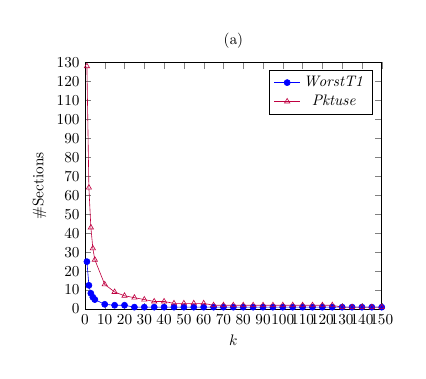
\begin{tikzpicture}[scale=0.55]
\begin{axis}[
    title={(a)},
    xlabel={$k$},
    ylabel={\#Sections},
    xmin=0, xmax=150,
    ymin=0, ymax=130,
    xtick={0,10,20,30,40,50,60,70,80,90,100,110,120,130,140,150},
    ytick={0,10,20,30,40,50,60,70,80,90,100,110,120,130},
    legend pos= north east,
    %ymajorgrids=true,
    grid style=dashed,
]
    \addplot[
    color=blue,
    mark=*,
    ]
    coordinates {
    (1,25)(2,12.5)(3,8.3)(4,6.25)(5,5)(10,2.5)(15,2)(20,2)(25,1)(30,1)(35,1)(40,1)(45,1)(50,1)(55,1)(60,1)(65,1)(70,1)(75,1)(80,1)(85,1)(90,1)(95,1)(100,1)(105,1)(110,1)(115,1)(120,1)(125,1)(130,1)(135,1)(140,1)(145,1)(150,1)
    };
    
      \addplot[
    color=purple,
    mark=triangle,
    ]
    coordinates {
    (1,128)(2,64)(3,43)(4,32)(5,26)(10,13)(15,9)(20,7)(25,6)(30,5)(35,4)(40,4)(45,3)(50,3)(55,3)(60,3)(65,2)(70,2)(75,2)(80,2)(85,2)(90,2)(95,2)(100,2)(105,2)(110,2)(115,2)(120,2)(125,2)(130,1)(135,1)(140,1)(145,1)(150,1)
    };    
    
    \legend{\textit{WorstT1},\textit{Pktuse}}
 
\end{axis}
 
\end{tikzpicture}
%\end{minipage}
%\begin{minipage}{.5\textwidth}
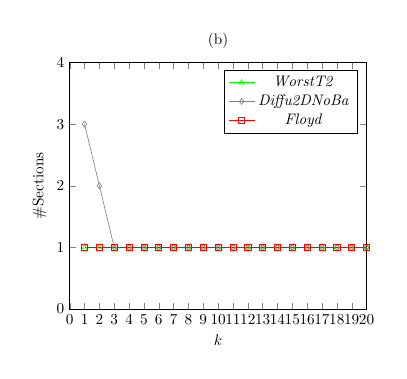
\begin{tikzpicture}[scale=0.55]
\begin{axis}[
title={(b)},
    xlabel={$k$},
    ylabel={\#Sections},
    xmin=0, xmax=20,
    ymin=0, ymax=4,
    xtick={0,1,2,3,4,5,6,7,8,9,10,11,12,13,14,15,16,17,18,19,20},
    ytick={0,1,2,3,4},
    legend pos= north east,
    %ymajorgrids=true,
    grid style=dashed,
]
     
\addplot[
    color=green,
    mark=triangle,
    ]
    coordinates {
    (1,1)(2,1)(3,1)(4,1)(5,1)(6,1)(7,1)(8,1)(9,1)(10,1)(11,1)(12,1)(13,1)(14,1)(15,1)(16,1)(17,1)(18,1)(19,1)(20,1)
    };
    
\addplot[
    color=gray,
    mark=diamond,
    ]
    coordinates {
    (1,3)(2,2)(3,1)(4,1)(5,1)(6,1)(7,1)(8,1)(9,1)(10,1)(11,1)(12,1)(13,1)(14,1)(15,1)(16,1)(17,1)(18,1)(19,1)(20,1)
    };
    
    \addplot[
    color=red,
    mark=square,
    ]
    coordinates {
        (1,1)(2,1)(3,1)(4,1)(5,1)(6,1)(7,1)(8,1)(9,1)(10,1)(11,1)(12,1)(13,1)(14,1)(15,1)(16,1)(17,1)(18,1)(19,1)(20,1)
    };
     
    
    \legend{\textit{WorstT2},\textit{Diffu2DNoBa},\textit{Floyd}}
 
\end{axis}
 
\end{tikzpicture}
%\end{minipage}
\caption{The number of partitioned sections of varying the input $k$.}
\label{fig:relation:section}
\end{figure}

\begin{figure}[!h]
\centering
%\begin{minipage}{.55\textwidth}
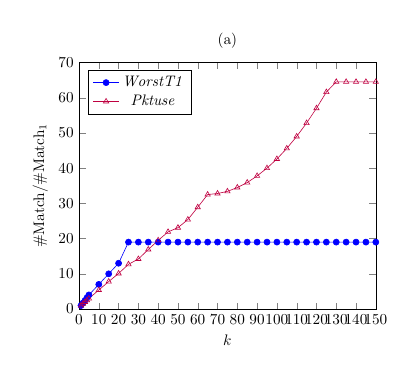
\begin{tikzpicture}[scale=0.55]
\begin{axis}[
   title = {(a)},
    xlabel={$k$},
    ylabel={\#Match$/$\#$\mathrm{Match}_1$},
    xmin=0, xmax=150,
    ymin=0, ymax=70,
    xtick={0,5,10,15},
    xtick={0,10,20,30,40,50,60,70,80,90,100,110,120,130,140,150},
    ytick={0,10,20,30,40,50,60,70},
    legend pos=  north west,
    %ymajorgrids=true,
    grid style=dashed,
]   

    
\addplot[
    color=blue,
    mark=*,
    ]
    coordinates {
    (1,1)(2,1.7)(3,2.4)(4,3.2)(5,4)(10,7)(15,10)(20,13)(25,19)(30,19)(35,19)(40,19)(45,19)(50,19)(55,19)(60,19)(65,19)(70,19)(75,19)(80,19)(85,19)(90,19)(95,19)(100,19)(105,19)(110,19)(115,19)(120,19)(125,19)(130,19)(135,19)(140,19)(145,19)(150,19)
    };
    

    
    \addplot[
    color=purple,
    mark=triangle,
    ]
    coordinates {
    (1,1)(2,1.5)(3,2)(4,2.5)(5,2.98)(10,5.4)(15,7.8)(20,10.1)(25,12.7)(30,14.2)(35,16.9)(40,19.5)(45,21.9)(50,23.1)(55,25.4)(60,28.9)(65,32.5)(70,32.8)(75,33.4)(80,34.5)(85,35.9)(90,37.8)(95,40)(100,42.6)(105,45.6)(110,49)(115,52.8)(120,57)(125,61.6)(130,64.5)(135,64.5)(140,64.5)(145,64.5)(150,64.5)
    };
    
    \legend{\textit{WorstT1},\textit{Pktuse}}
\end{axis}
\end{tikzpicture}
%\end{minipage}
%\begin{minipage}{.55\textwidth}
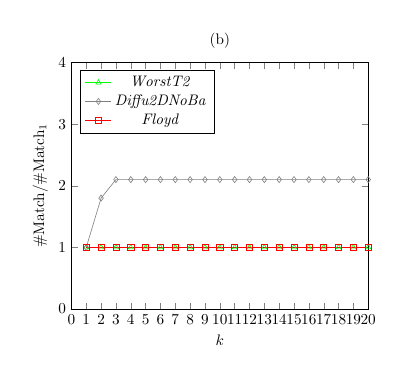
\begin{tikzpicture}[scale=0.55]
\begin{axis}[
   title = {(b)},
    xlabel={$k$},
    ylabel={\#Match$/$\#$\mathrm{Match}_1$},
    xmin=0, xmax=20,
    ymin=0, ymax=4,
    xtick={0,5,10,15},
    xtick={0,1,2,3,4,5,6,7,8,9,10,11,12,13,14,15,16,17,18,19,20},
    ytick={0,1,2,3,4},
    legend pos=  north west,
    %ymajorgrids=true,
    grid style=dashed,
]   
    
     %\addplot[
    %color=red,
   % mark=square,
    %]
    %coordinates {
%(1,1)(2,1)(3,1)(4,1)(5,1)(10,1)(15,1)(20,1)(25,1)(30,1)(35,1)(40,1)(45,1)(50,1)(55,1)(60,1)(65,1)(70,1)(75,1)(80,1)(85,1)(90,1)(95,1)(100,1)(105,1)(110,1)(115,1)(120,1)(125,1)(130,1)(135,1)(140,1)(145,1)(150,1)
 %   };
    
    \addplot[
    color=green,
    mark=triangle,
    ]
    coordinates {
    (1,1)(2,1)(3,1)(4,1)(5,1)(6,1)(7,1)(8,1)(9,1)(10,1)(11,1)(12,1)(13,1)(14,1)(15,1)(16,1)(17,1)(18,1)(19,1)(20,1)(25,1)(30,1)(35,1)(40,1)(45,1)(50,1)(55,1)(60,1)(65,1)(70,1)(75,1)(80,1)(85,1)(90,1)(95,1)(100,1)(105,1)(110,1)(115,1)(120,1)(125,1)(130,1)(135,1)(140,1)(145,1)(150,1)
    };
    
    \addplot[
    color=gray,
    mark=diamond,
    ]
    coordinates {
    (1,1)(2,1.8)(3,2.1)(4,2.1)(5,2.1)(6,2.1)(7,2.1)(8,2.1)(9,2.1)(10,2.1)(11,2.1)(12,2.1)(13,2.1)(14,2.1)(15,2.1)(16,2.1)(17,2.1)(18,2.1)(19,2.1)(20,2.1)(25,2.1)(30,2.1)(35,2.1)(40,2.1)(45,2.1)(50,2.1)(55,2.1)(60,2.1)(65,2.1)(70,2.1)(75,2.1)(80,2.1)(85,2.1)(90,2.1)(95,2.1)(100,2.1)(105,2.1)(110,2.1)(115,2.1)(120,2.1)(125,2.1)(130,2.1)(135,2.1)(140,2.1)(145,2.1)(150,2.1)
    };
    
    \addplot[
    color=red,
    mark=square,
    ]
    coordinates {
    (1,1)(2,1)(3,1)(4,1)(5,1)(6,1)(7,1)(8,1)(9,1)(10,1)(11,1)(12,1)(13,1)(14,1)(15,1)(16,1)(17,1)(18,1)(19,1)(20,1)(25,1)(30,1)(35,1)(40,1)(45,1)(50,1)(55,1)(60,1)(65,1)(70,1)(75,1)(80,1)(85,1)(90,1)(95,1)(100,1)(105,1)(110,1)(115,1)(120,1)(125,1)(130,1)(135,1)(140,1)(145,1)(150,1)
    };
    
    \legend{\textit{WorstT2},\textit{Diffu2DNoBa},\textit{Floyd}}
\end{axis}
\end{tikzpicture}
%\end{minipage}

\caption{The relative growth of the number of match pairs of varying the input $k$, where $\mathrm{Match}_1$ is the number of the generated match pairs for $k=1$.}
\label{fig:relation:match}
\end{figure}


\end{comment}

The first benchmark, \textit{WorstT1}, is constructed by restricting all the receives in \figref{fig:Texample} to be wildcard, which implies the worst case of message non-determinism. In contrast, the best case of message non-determinism is a program that only contains deterministic receives. Thus, the matches for the best case program are deterministic. Also, let $m=4$ and $|S| = 25$ in the program configuration. 

%In contrast, the second benchmark \textit{BestT1} is the best case of message non-determinism, where the program text is similar to \textit{WorstT1} only the receives are deterministic. 


The second benchmark, \textit{WorstT2}, is related to the worst case of wide communication. Wide communication in this context means that the sender only sends one message to the receiver. The program is constructed by setting $|S|=1$ and $m=100$. As for the best case of wide communication, the program has to contain only the deep communication where a receiver has exactly one sender. The matches for this type of best case are deterministic because the sends from the identical sender can only match the receives in the receiver in a non-overtaking order. 

Given the two worst-case programs, the presentation discusses how the number of sections and the number of match pairs grow as $k$ increases for the two programs. 
The relationship between the number of sections and $k$ is illustrated in \figref{fig:relation:section}, and the relationship between the number of match pairs and $k$ is illustrated in \figref{fig:relation:match}.
Note that the values of y-axis in \figref{fig:relation:match} are computed by dividing the number of match pairs for any $k$ by the number of match pairs for $k=1$.

\figref{fig:relation:section} (a) shows that the reduction of the number of sections is not linear for the program \textit{WorstT1}, and incrementing $k$ may not be meaningful if the number of sections does not change. The algorithm in this paper only increments $k$ until the number of sections changes, and then outputs the generated match pairs with $k$ to the SMT encoding.
Since the number of the generated match pairs per section is also non-linear,
%according to the complexity of the existing algorithm \cite{DBLP:conf/kbse/HuangMM13}, 
the total number of the match pairs for \textit{WorstT1} in \figref{fig:relation:match} (a) has a sharp growth between small values of $k$, and then grows more gently until it reaches the bound, which represents the over-approximated match pairs. This observation demonstrates that the algorithm scales for a small range of $k$ where the generated match set is small.

%The program \textit{BestT1} has the same growth of the number of sections with that for \textit{WorstT1} (not shown in \figref{fig:relation} (a)) because the send distribution has no difference between the two programs. 
%Since all the receives are deterministic in the program \textit{BestT1} indicating the matches are also deterministic, the number of the match pairs in \figref{fig:relation} (b) does not grow across $k$.

For the program \textit{WorstT2}, \figref{fig:relation:section} (b) shows that the number of sections is always one as expected because only one section can be partitioned for wide communication. 
Therefore, the total number of match pairs for \textit{WorstT2} in \figref{fig:relation:match} (b) does not change. 

Based on the discussion of message non-determinism and wide communication, the programs discussed earlier can be grouped. The programs \textit{DeepComm}, \textit{MultiM} are close to the worst case of message non-determinism as only wildcard receives are employed in both programs. For wide communication, \textit{Floyd}, \textit{Integrate} and \textit{IS} are close to the worst case. Therefore, their growths in \figref{fig:relation:match} rapidly reach the bound of match pairs, which means the time costs for those programs are not improved by the under-approximation approach. 
In contrast, the other programs have a certain degree of deep communication. For example, \textit{Pktuse} employs a high degree of deep communication with many wildcard receives. As such, \textit{Pktuse} in \figref{fig:relation:match} (a) gradually grows to the bound as $k$ increases to $128$.
\textit{Mismatch}, \textit{MismatchEx}, \textit{MonteCarlo} and \textit{Heat} in \figref{fig:relation:match} also show gradual growths. 
As such, the property witnessing for those programs reaches a speedup as shown in \tableref{table:benchmarks}.

In summary, the scalability tests demonstrate that our under-approximation approach is able to scale to a program with a high degree of message non-determinism and/or a high degree of deep communication.


\begin{comment}
The real programs can also be classified for message non-determinism and wide communication. \figref{fig:relation:section} and \figref{fig:relation:match} further plot the growths for the real programs. 
The programs \textit{Diffu2DNoBa} and \textit{Floyd} uses more wide communication, therefore, their growths in \figref{fig:relation:match} rapidly reach the bound of match pairs. In contrast, the program \textit{Pktuse} employs a high of deep communication with many wildcard receives. As such, \textit{Pktuse} in \figref{fig:relation:match} (a) gradually grows to the bound as $k$ increases to $128$.
Therefore, the presentation demonstrates that our algorithm is able to scale to a program with a high degree of message non-determinism and a high degree of deep communication.

\end{comment}


